\section{Latent Intellectual Communities in a Research Institution}
\label{sec:Q}
Does a research institution harbour latent intellectual communities whose members work on related problems without directly engaging with each other's work---and can such communities be surfaced from publication records alone?

Citation is a selective and socially shaped practice: researchers cite work they know, and knowledge often travels within established collaboration networks rather than across them. Furthermore, institutional boundaries do not automatically generate awareness: two groups within the same university may develop parallel research programmes in isolation, connected only through shared reference pools rather than through direct intellectual exchange. When both phenomena operate simultaneously, the citation graph will systematically underrepresent the true intellectual proximity within the institution.

\subsection{BC-corrected communities and localisation of gaps}
\label{subsec:q:bccorr}

We started from structural convergence: if hyperedge co-occurrence and bibliographic coupling capture the same latent signal, gap candidates should localise in precisely those communities that BC \emph{corrects}---communities that appear disconnected under pure citation but merge when external references are added.

On $G_\text{CitOnly}$, the three algorithms produce approximately the same number of communities (with different properties and characteristics; see \ref{sec:CD}), but the $G_\text{BC}$ effect diverges across algorithms, each fusing a different share of communities (Table~\ref{tab:bccorr}). 

% TODO – CONTESTO MANCANTE
% Questa frase apre il risultato principale di Sezione 6 ma risulta decontestualizzata. Prima di essa occorre:
%   1. Ricordare brevemente la distinzione fused/stable (definita in Sec. 4)
%   2. Motivare la scelta di top-200 (vs top-100 usato in Table 9)
%   3. Aggiungere una frase di transizione tipo:
%      "To test whether gap candidates localise in structurally corrected regions of the graph, for each of the 200 top-ranked debiased gap candidates (Section 5) we record..."
% In alternativa, spostare la definizione di fused/stable in un mini-reminder inline: "...fused community (one in which BC merged two or more G_{CitOnly} communities) or a stable one (unchanged by BC)..."

To test whether gap candidates localise in structurally corrected regions of the graph, for each of the 200 top-ranked debiased gap candidates obtained in Hypeergraph analysis (Section 5) we record whether its two nodes land in the same $G_\text{BC}$ community, and whether that community is \textbf{fused} (one in which BC merged two or more $G_\text{CitOnly}$ communities) or \textbf{stable} (membership unchanged by BC).

\begin{table}[h]
\centering
\begin{tabular}{lccc}
\toprule
Algorithm & G$_\text{CitOnly}$ comms & Fused comms \\
\midrule
Leiden & 1\,533 & 68   \\
InfoMap & 1\,496 & 46   \\
ANGEL (crisp) & 1\,526 & 355  \\
\bottomrule
\end{tabular}
\smallskip
\caption{Fused communities in $G_\text{BC}$. For ANGEL, any $G_\text{CitOnly}$ community in an overlap counts as fused; the higher count reflects boundary sensitivity rather than structural change.}
\label{tab:bccorr}
\end{table}


All 200/200 gap candidates fall in fused communities---a design consistency check rather than a discovery: no candidate drifts into the 7.6\% of nodes where BC leaves the partition unchanged, which would signal a malfunction of the scoring function.

The interpretation is structural: BC and the hypergraph converge on the same latent communities at two different scales.  BC (macro level) identifies where citation has \emph{fragmented} an intellectually coherent group---the 68 fused communities.  The hypergraph (micro level) identifies \emph{which specific pairs} within those corrected groups share references without citing each other.  %[REVISED: removed redundant tail clause that restated the preceding independent clause]
The 930 stable communities produce zero gap candidates: citation had already drawn those boundaries correctly.

The remaining analyses (§§\ref{subsec:q:conv}--\ref{subsec:q:neardup}) use the top-100 shortlist, the subset subjected to manual title inspection, topic classification, and temporal analysis.  The full top-200 pool serves only the automated BC-localisation check above; rank-band validation (\S\ref{subsec:q:conv}) confirms same-community rates of 100\% for ranks~1--150 and 96\% for ranks~151--200, validating top-100 as the high-confidence working set.

\subsection{Cross-Algorithm Convergence}
\label{subsec:q:conv}
For each of the top~100 debiased gap candidates we check whether both
nodes belong to the same community under each of the four
algorithm-graph configurations.  Figure~\ref{fig:cross_algo}
reports the results alongside random baselines computed over 2\,000
uniformly sampled uncited node pairs.

The Leiden $G_\text{CitOnly}$ control already reaches 99\%---hyperedge
co-occurrence is itself a strong intra-community signal, independent of
BC restructuring.  Adding BC edges lifts Leiden to 100\%; InfoMap and
ANGEL both confirm 100\%.

The enrichment factor varies by two orders of magnitude---from
$5.3\times$ (InfoMap) to $83.3\times$ (ANGEL)---reflecting differences
in partition granularity, not in the underlying signal.  InfoMap's high
baseline (18.8\%) is a consequence of the $\approx$23\,000-node
super-community identified in Section~\ref{sec:CD}.  ANGEL, which
distributes ambiguous nodes across multiple communities, yields the
cleanest enrichment because its crisp projection produces many small
communities (median size~10 on~$G_\text{BC}$) and thus a very low
baseline.

Bootstrap validation (2,000 draws of 100 random uncited pairs, Leiden)
gives a null mean of 7.2\%, never exceeding 16\%; gap candidates achieve
100\% ($p < 0.0005$, minimum reportable with 2,000 replicates).
Stratifying by rank band, the same-community rate is stable: 100\% for
ranks~1--150 and 96\% for ranks~151--200.

\begin{figure}[t]
\centering
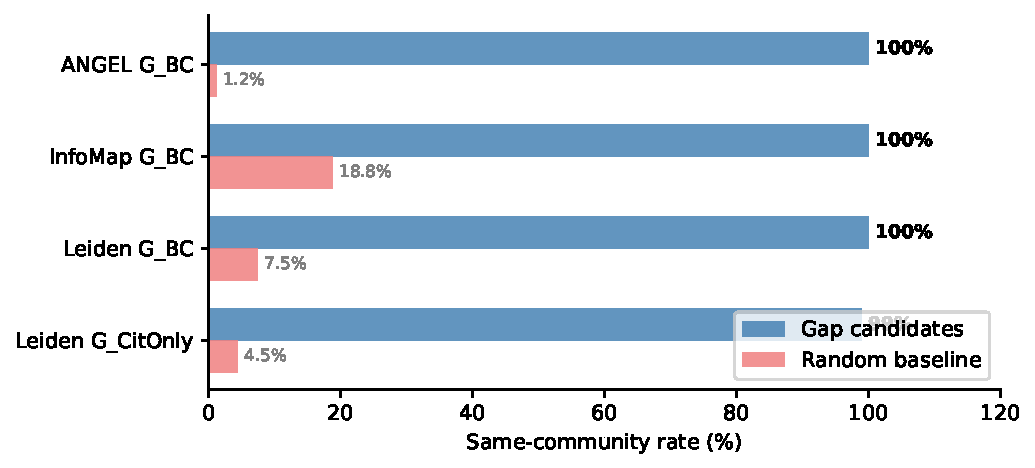
\includegraphics[width=0.45\textwidth]{img/cross_algo_robustness.pdf}
\caption{Same-community rate for the top-100 gap candidates vs.\ random
baseline (fraction of random uncited pairs sharing a community), under
four algorithm-graph configurations.  The $G_\text{CitOnly}$ bar is the
no-BC control.}
\label{fig:cross_algo}
\end{figure}

%-----------------------------------------------------------------------
\subsection{Disciplinary and Thematic Profile of Gap Candidates}
\label{subsec:q:discip}
%-----------------------------------------------------------------------

%[REVISED: merged §Topic Cluster Analysis into §Disciplinary Identity; subsection header eliminated; opening trimmed; LLM sentence dissolved into topic paragraph as transition]
Despite spanning 55\,078 UniPi nodes, the 100 top gap candidates
concentrate in only 6 of the 1\,210 $G_\text{BC}$ communities
(Figure~\ref{fig:community_profile}).  Five exhibit at least 60\%
FOS~L4 sub-discipline purity; the sixth (C3, Chemical sciences)
reaches only 45\% (Table~\ref{tab:comms}).  At the pair level, 81 of
100 share the same four-digit FOS code; the remaining~19 lack a tag on
one side but are confirmed same-topic by title
inspection---consistent with the finding in Section~\ref{sec:HG} that
72\% of the top-50 gap candidates share an FOS~L2 domain.

\begin{table}[h]
\centering
\small
\begin{tabular}{lrrll}
\toprule
C & Size & Gap pairs & Dominant FOS~L4 & Purity \\
\midrule
C8  & 2\,074 & 53 & 0103 Physical sciences  & 79\% \\
C0  & 9\,145 & 30 & 0302 Clinical medicine  & 60\% \\
C7  & 2\,693 & 10 & 0103 Physical sciences  & 60\% \\
C5  & 3\,340 &  4 & 0302 Clinical medicine  & 64\% \\
C3  & 4\,817 &  2 & 0104 Chemical sciences  & 45\% \\
C11 & 1\,356 &  1 & 0103 Physical sciences  & 68\% \\
\bottomrule
\end{tabular}
\caption{$G_\text{BC}$ communities (Leiden) hosting gap candidates.
Purity = fraction of nodes sharing the dominant FOS~L4 sub-discipline.}
\label{tab:comms}
\end{table}

Title-level classification by an LLM (Claude Opus 4.6), verified by
manual inspection,\footnote{Standard text-clustering pipelines
(TF-IDF, BERTopic) were inadequate on this dataset: OpenAIRE keyword
fields are sparsely populated and inconsistently formatted, producing
degenerate clusters.  LLM-assisted classification was adopted as a
pragmatic alternative.} confirms 95 genuine gap pairs among the
top-100 candidates (5 near-duplicates; see
Section~\ref{subsec:q:neardup}).  The two dominant clusters are
gravitational-wave and astrophysics research (47 pairs, 33 unique
UniPi nodes, publications spanning 2010--2024) and
diabetes/cardiovascular medicine (18 pairs).  Smaller clusters cover
HEP/particle physics (9~pairs), thyroid and endocrine disorders (5),
and oncology (4); the remainder spans vascular surgery, rheumatology,
and 8~pairs without a domain label (Figure~\ref{fig:topic_clusters}).

\begin{figure}[t]
\centering
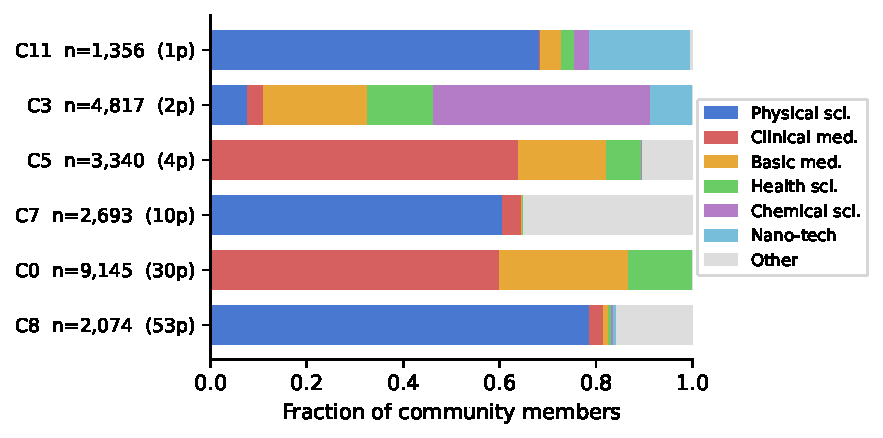
\includegraphics[width=0.45\textwidth]{img/community_fos_profile.pdf}
\caption{Disciplinary composition of the 6 $G_\text{BC}$ communities
hosting gap candidates (Leiden).}
\label{fig:community_profile}
\end{figure}

The GW/astrophysics cluster is the clearest example of a
\emph{citation-invisible} community that the pipeline recovers from
bibliographic records alone---and thereby validates its own
sensitivity.  Thirty-three UniPi nodes contribute to the Einstein
Telescope and LIGO/Virgo collaborations: they share dense reference
overlap, publish in overlapping venues, and work on the same detector
physics.  In mega-collaborations of this scale, researchers co-author
experiment-wide papers and share data pipelines; the members know each
other, so their proximity is not sociologically latent. It is,
however, \emph{invisible in the internal citation graph}: cross-unit
citation is not how collaborative output is recorded.  The GW case
thus serves as a \emph{positive control}: a community whose existence
is independently known and that the pipeline correctly identifies.
The diabetes/cardiovascular and HEP clusters (18 and 9~pairs
respectively), where researchers are less likely to know each other
through shared collaboration structures, are stronger candidates for
the ``latent'' label.
\begin{figure}[h]
\centering
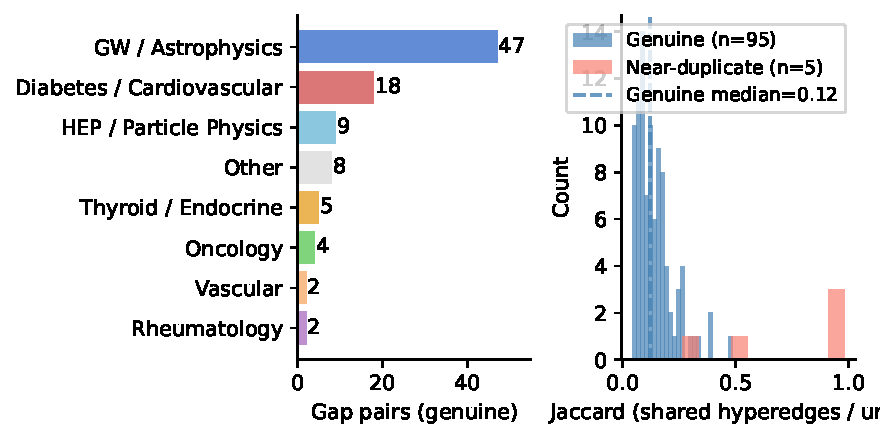
\includegraphics[width=0.45\textwidth]{img/topic_clusters.pdf}
\caption{Distribution of the 95 genuine gap pairs across topic clusters.}
\label{fig:topic_clusters}
\end{figure}

\subsection{What Bibliographic Coupling Adds to the Hyperedge Signal}
\label{subsec:q:hevsbc}

An ablation study compares the top-50 gap candidates produced by three
scoring regimes on the same graph: (A)~hyperedge-debiased
score~\eqref{eq:debias} alone; (B)~BC-weight score alone (raw
bibliographic-coupling edge weight, no degree correction); and (C)~the
full combined pipeline.  The overlap between regimes~A and~B is zero:
$|\text{top-50}_A \cap \text{top-50}_B| = 0$.

Regime~B without degree correction is dominated by pairs with BC-weight
exactly~1.0 and degree~$\approx 1.3$---supplementary files of the same
paper, which share a single external reference and have virtually no
other connections.  These are artefacts of document fragmentation in
the OpenAIRE metadata, not collaboration gaps.  Regime~A, by contrast,
surfaces pairs with mean degree~$\approx 53$ and a mean of 344 shared
hyperedges---papers well-embedded in the citation network with a broad
reference context.

%[REVISED: two conflated facts (A∩C and B∩C) separated into explicit statements; inline formula removed and replaced with prose]
Regimes~A and~C share 47 of their respective top-50 pairs, confirming that HE-debiased scoring drives the combined pipeline. Regime~B contributes none of those top-50: its candidates are entirely displaced by artefacts and do not survive into the combined ranking.  BC's contribution is structural rather than ranking-based: BC-corrected community assignments provide the localisation context within which HE-ranked pairs are validated.  HE identifies \emph{which} pairs share thematic context; BC identifies \emph{where} in the community structure those pairs sit.

\subsection{Temporal Structure of Gap Candidates}
\label{subsec:q:temporal}

The 100 gap candidates distribute across three temporal categories:
69~pairs in which both nodes were published before 2020
(\emph{Parent--Parent}), 22~pairs in which one node is recent
($\geq 2020$) and the other is not (\emph{Recent--Parent}), and
9~pairs in which both nodes are recent (\emph{Recent--Recent}).
The median year gap within a pair is 2~years (mean~3.3, max~13);
18~pairs share the same publication year.  Spearman
$\rho(\text{score},\,\text{year gap}) = -0.14$ ($p = 0.16$,
n.s.)---the gap score is not biased toward temporally distant pairs.

The dominant gap type is not ``two contemporaneous researchers who are
unaware of each other'' but rather ``two papers---often from different
UniPi generations---that share intellectual context without direct
citation.''  For operational purposes, the 9~Recent--Recent pairs
carry the strongest collaboration plausibility; applying the
near-duplicate filter (Section~\ref{subsec:q:neardup}) reduces this
to 7~genuine pairs: 6 within the GW/astrophysics community and
1~HEP pair (score~$= 7.58$, Jaccard~$= 0.49$) representing two
particle-physics groups sharing a broad reference context without
any direct citation.  The 22~Recent--Parent pairs may identify cases
where a current researcher has not cited a still-active older
colleague.  The 69~Parent--Parent pairs document historical thematic
proximity with limited immediate actionability.


\subsection{Near-Duplicate Detection}
\label{subsec:q:neardup}

Among the top-100 candidates, 3 pairs are removed by a Jaccard
similarity threshold of $\geq 0.70$ on their shared-hyperedge sets;
2 further pairs, with $J = 0.265$ and $J = 0.520$, are flagged by
manual inspection as same-paper duplicates published in different
venues (e.g., an ESC consensus statement appearing in two journals,
or a LIGO paper appearing as both a preprint and a journal article).
All 5 are excluded from the topic and temporal analyses above and
flagged in the exported candidate list as a sensitivity signal.

These cases survive OpenAIRE deduplication~\cite{openaire_dedup},
which does not resolve deliberate multi-venue publications where
records are genuinely distinct in provenance.  A production deployment
would benefit from a pre-filter based on title similarity or DOI
crosswalk, applied \emph{before} hyperedge construction.
